\section{Модификация проекта «Выпуклая оболочка»}

\subsection{Постановка задачи}

Модифицируйте эталонный проект таким образом, чтобы вычислялось количество пар вершин выпуклой оболочки, расстояние между которыми не превосходит единицу.
На начальном этапе работы программа запрашивает координаты вершин выпуклой оболочки, которая впоследствии индуктивно добавляет ее в выпуклую оболочку. Для решения нашей задачи необходимо выводить, помимо значений периметра и площади, количество пар вершин выпуклой оболочки, расстояние между которыми не превосходит единицу.

Для выполнения задания необходимо обладать базовыми знаниями в линейной алгебре. 2 точки, при их соединении, образуют отрезок, который можно представить в виде вектора. Чтобы получить длину (модуль) вектора $\overrightarrow{AB}$ необходимо воспользоваться следующей формулой:
$$\mid \overrightarrow{AB} \mid = \sqrt{(B_{x}-A_{x})^2+(B_{y}-A_{y})^2}$$  

Рассмотрим пример. Для последовательности точек $A(0, 0)$, $B(1, 0)$ и $C(0, 5)$ программа
выводит 1 в качестве количествa пар, расстояние между которыми не превосходит единицу.
После того,как мы вели  следующую точку $D(1, 5)$, количество ребер, расстояние между которыми не превосходит единицу, равняется $2$ (рис.~1).

\begin{figure}[ht!]
\begin{center}
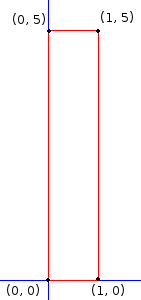
\includegraphics[scale=0.7]{images/picture1}
\center{\texttt{Рис.~1.}}
\end{center}
\end{figure}
\newpage

\sloppy Все требуемые функции будут вписываться в файлы проекта \texttt{convex.rb} и \texttt{r2point.rb}.

\subsection{Решение}

Для выполнения задания необходимо вычислять растояние между вершинами выпуклой оболочки. В эталонном проекте изначально присутствует функция \texttt{dist}, которая считает расстояние между вершинами выпуклой оболочки.
\subsection{Модификация кода}
При реализации кода были произведены изменения в четырех файлах эталонного проекта: \texttt{r2point.rb}, \texttt{convex.rb}, \texttt{run\_convex.rb}, \texttt{run\_tkconvex.rb}.
Рассмотрим  изменения кода в файле \texttt{r2point.rb}. В него был добавлен метод \texttt{distance}:

\begin{small}
\begin{verbatim}
class R2Point
...
  def distance(a)
    return (self.dist(a)<=1)? 1 : 0
  end
  ...
\end{verbatim}
\end{small}

Данный метод рассматривает две точки, и проверяет, не превышает ли расстояние между вершинами $1$. Для этого используется метод \texttt{dist} класса \texttt{R2Point}  В случае, если расстояние меньше либо равно единице, то метод \texttt{distance} возвращает значение 1, в противном случае, возвращается 0. На этом модификация файла \texttt{r2point.rb} завершена.
\newpage
Рассмотрим модификацию файла \texttt{convex.rb}. В классе \texttt{Segment} добавляется метод \texttt{dist}:

\begin{small}
\begin{verbatim}
class Segment < Figure
  ...
  def dist
    return (@p.dist(@q) <= 1)? 1 : 0
  end
  ...
\end{verbatim}
\end{small}

Этот метод проверяет длину двуугольника (отрезка). Если она больше единицы возвращается значение 0, иначе возвращается значение 1.

Затем редактируется класс \texttt{Polygon}. Первоначально при создании объекта класса \texttt{Polygon} создается треугольник. Необходимо при инициализации объекта посчитать расстояния между вершинами треугольника и узнать, сколько пар вершин, между которыми расстояние не более единицы.

\begin{small}
\begin{verbatim}
class Polygon < Figure
  attr_reader :points, :perimeter, :area

  def initialize(a, b, c)
    ...
    @dist = a.distance(b) + b.distance(c) + c.distance(a)
  end
  ...
\end{verbatim}
\end{small}

В последстви, при добавлении новых точек индуктивно вычисляется расстояние от добавляемой точки, до первой и последней вершин выпуклой облочки :

\begin{small}
\begin{verbatim}
  ...
  @perimeter += t.dist(@points.first) + t.dist(@points.last)
  @dist += t.distance(@points.first) + t.distance(@points.last)
  @points.push_first(t)
  ...
\end{verbatim}
\end{small}

Как и при добавлени, так и при удалении вычисляется расстояние между вершинами, и если расстояние между парами вершин превышает $1$, то удаляются из переменной.

\begin{small}
\begin{verbatim}
 p = @points.pop_first
   while t.light?(p, @points.first)
     @perimeter -= p.dist(@points.first)
     @area      += R2Point.area(t, p, @points.first).abs
     @dist      -= p.distance(@points.first)
     p  = @points.pop_first
   end
 @points.push_first(p)
  ...
  p = @points.pop_last
    while t.light?(@points.last, p)
      @perimeter -= p.dist(@points.last)
      @area      += R2Point.area(t, p, @points.last).abs
      @dist      -= p.distance(@points.last)
      p = @points.pop_last
    end
  @points.push_last(p)
\end{verbatim}
\end{small}

Далее расмотрим примеры работы программы. 
В случае, когда создается объект класса \texttt{Void} количество вершин выпуклой оболочки равно нулю. Когда добавляется вершина создается объект класса \texttt{Point}. В обоих случаях количество вершин оболочки меньше двух, считать расстояние между вершинами невозможно и возвращается число 0. При создании объектов классов \texttt{Segment} и \texttt{Polygon} количество вершин больше либо равно двум и необходимо считать расстояния между вершинами.
Для точек  с координатами$(0, 0)$ и $(1, 0)$ расстояние между которыми равно 1, следовательно, программа выведет 1 (рис.~2).

\begin{figure}[ht!]
\begin{center}
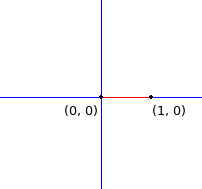
\includegraphics[scale=1.0]{images/picture2.png}
\center{\texttt{Рис.~2.}}
\end{center}
\end{figure}
\newpage
При добавелнии новой точки $(0, 1)$, расстояние между всеми точками пересчитывается, и программа выводит результат 2. Так как растояние между вершинами $(0, 0)$ и $(0, 1)$, $(0, 0)$ и $(1, 0)$ равно 1, а расстояние между вершинами $(0, 1)$ и $(1, 0)$ превосходит 1 (рис.~3).

\begin{figure}[ht!]
\begin{center}
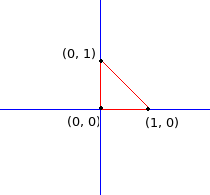
\includegraphics[scale=1.0]{images/picture3.png}
\center{\texttt{Рис.~3.}}
\end{center}
\end{figure}


При добавлении точки $(1, 1)$, программа пересчитывает расстояния между точками и выводит ответ $4$ (рис.~4).

\begin{figure}[ht!]
\begin{center}
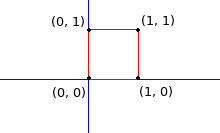
\includegraphics[scale=1.0]{images/picture4.png}
\center{\texttt{Рис.~4.}}
\end{center}
\end{figure}

\newpage
Далее добавляется новая точка $(1, 3)$. Точка $(1, 1)$ удаляется и выводится ответ 2 (рис.~5).

\begin{figure}[ht!]
\begin{center}
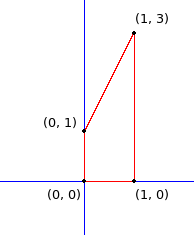
\includegraphics[scale=1.0]{images/picture5.png}
\center{\texttt{Рис.~5.}}
\end{center}
\end{figure}

